% ============================================================================
% Artigo: Salto Tecnologico: BeeGe
% Autor: Gabriel Monteiro
% Programa: NaPratica (Modulo de Empreendedorismo)
% Para compilar: pdflatex ou Overleaf (engine: pdfLaTeX)
% ============================================================================

\documentclass[12pt, a4paper]{article}

% ── Pacotes ──────────────────────────────────────────────────────────────────
\usepackage[utf8]{inputenc}
\usepackage[T1]{fontenc}
\usepackage[brazilian]{babel}
\usepackage{lmodern}
\usepackage{geometry}
\usepackage{setspace}
\usepackage{indentfirst}
\usepackage{graphicx}
\usepackage{float}
\usepackage{url}
\usepackage{booktabs}
\usepackage{array}
\usepackage{tabularx}
\usepackage{longtable}
\usepackage{enumitem}
\usepackage{amsmath, amssymb}
\usepackage{xcolor}
\usepackage{tikz}
\usetikzlibrary{positioning}
\usepackage{titlesec}
\usepackage{fancyhdr}
\setlength{\headheight}{14pt}
\usepackage{caption}
\usepackage{subcaption}
\usepackage{tcolorbox}
\tcbuselibrary{skins}
\usepackage[plainpages=false,pdfpagelabels]{hyperref}

% ── Configuracoes de pagina ─────────────────────────────────────────────────
\geometry{
  top=3cm,
  bottom=2cm,
  left=3cm,
  right=2cm
}
\setstretch{1.5}

% ── Cores do projeto ────────────────────────────────────────────────────────
\definecolor{beegeAmbar}{HTML}{F59E0B}
\definecolor{beegePurple}{HTML}{7C3AED}
\definecolor{beegeGray}{HTML}{374151}

% ── Estilo de cabecalho e rodape ────────────────────────────────────────────
\pagestyle{fancy}
\fancyhf{}
\fancyhead[L]{\small\textcolor{beegeGray}{BeeGe | Salto Tecnol\'{o}gico}}
\fancyhead[R]{\small\textcolor{beegeGray}{NaPr\'{a}tica 2026}}
\fancyfoot[C]{\thepage}
\renewcommand{\headrulewidth}{0.4pt}

% ── Estilo de secoes ───────────────────────────────────────────────────────
\titleformat{\section}
  {\Large\bfseries\color{beegePurple}}{\thesection}{1em}{}
\titleformat{\subsection}
  {\large\bfseries\color{beegeGray}}{\thesubsection}{1em}{}
\titleformat{\subsubsection}
  {\normalsize\bfseries\color{beegeGray}}{\thesubsubsection}{1em}{}

% ── Caixa de destaque ──────────────────────────────────────────────────────
\newtcolorbox{destaque}[1][]{
  colback=beegeAmbar!10,
  colframe=beegeAmbar,
  fonttitle=\bfseries,
  title={#1},
  arc=3pt,
  boxrule=0.8pt
}

% ── Hyperlinks ─────────────────────────────────────────────────────────────
\hypersetup{
  colorlinks=true,
  linkcolor=beegePurple,
  urlcolor=beegePurple,
  citecolor=beegePurple
}

% ============================================================================
%                           INICIO DO DOCUMENTO
% ============================================================================
\begin{document}
\hypersetup{pageanchor=false}

% ── Capa Executiva ──────────────────────────────────────────────────────────
\begin{titlepage}
\thispagestyle{empty}
\begin{center}
    % Faixa superior
    \begin{tcolorbox}[
        colback=beegePurple,
        colframe=beegePurple,
        arc=4pt,
        boxrule=0pt,
        width=\textwidth,
        halign=center,
        top=8pt,
        bottom=8pt
    ]
        {\small\color{white}\bfseries PROGRAMA NAPR\'{A}TICA \;\textcolor{white!70}{$\bullet$}\; M\'{O}DULO DE EMPREENDEDORISMO}
    \end{tcolorbox}
    
    \vspace{20pt}

    % Mascote Limia centralizado
    
\includegraphics[width=3.6cm, keepaspectratio]{assets/limia.png}
    
    \vspace{14pt}

    % Nome do Produto e Slogan
    {\fontsize{32}{38}\selectfont\bfseries\textcolor{beegePurple}{BeeGe}}\\[10pt]
    {\fontsize{18}{23}\selectfont\bfseries\textcolor{beegeGray}{Plataforma Gamificada de Revis\~{a}o de C\'{a}lculo~1}}\\[8pt]
    {\large\textcolor{beegeGray!70}{Um app para estudantes revisarem C\'{a}lculo de forma pr\'{a}tica e engajante}}

    \vspace{20pt}

    % Caixa de Destaque do Relatorio
    \begin{tcolorbox}[
        colback=beegeAmbar!8,
        colframe=beegeAmbar,
        arc=4pt,
        boxrule=1.2pt,
        width=0.92\textwidth,
        halign=center,
        top=8pt,
        bottom=8pt
    ]
        {\large\bfseries\textcolor{beegeGray}{RELAT\'{O}RIO: SALTO TECNOL\'{O}GICO}}\\[4pt]
        {\small\textcolor{beegeGray!85}{Da ideia ao produto funcionando em 30 dias (20/09 a 19/10/2026)}}
    \end{tcolorbox}

    \vspace{18pt}

    % Cartao de Metadados
    \begin{tcolorbox}[
        colback=white,
        colframe=beegePurple!30,
        arc=4pt,
        boxrule=0.9pt,
        width=0.94\textwidth,
        left=14pt,
        right=14pt,
        top=10pt,
        bottom=10pt
    ]
        \renewcommand{\arraystretch}{1.35}
        \centering
        \begin{tabular}{r @{\hspace{10pt}} l}
            \textbf{\textcolor{beegePurple}{Autor:}} & Gabriel Monteiro \\[2pt]
            \textbf{\textcolor{beegePurple}{\'{A}rea:}} & Engenharia de Software \\[2pt]
            \textbf{\textcolor{beegePurple}{Reposit\'{o}rio:}} & \href{https://github.com/GabrielSMonteiro/Calculus}{\small\texttt{github.com/GabrielSMonteiro/Calculus}} \\[2pt]
            \textbf{\textcolor{beegePurple}{V\'{i}deo Demonstrativo:}} & \href{https://youtu.be/lCUiceX9FIk}{\small\texttt{youtu.be/lCUiceX9FIk}}
        \end{tabular}
    \end{tcolorbox}

    \vfill

    % Rodape da Capa
    \textcolor{beegePurple!30}{\rule{0.5\textwidth}{0.8pt}}\\[8pt]
    {\small\bfseries\textcolor{beegeGray}{Bras\'{i}lia $\cdot$ DF}\\[2pt]
    \small\textcolor{beegeGray!75}{Outubro de 2026}}
    \vspace*{-0.2cm}
\end{center}
\end{titlepage}

% ── Sumario ─────────────────────────────────────────────────────────────────
\newpage
\hypersetup{pageanchor=true}
\pagenumbering{roman}
\setcounter{page}{2}
\thispagestyle{empty}
{
  \hypersetup{linkcolor=beegePurple}
  \renewcommand{\contentsname}{\vspace*{-1.4cm}\LARGE\bfseries\textcolor{beegePurple}{Sum\'{a}rio}\vspace{4pt}}
  \setlength{\parskip}{0pt}
  \begin{spacing}{0.84}
    \tableofcontents
  \end{spacing}
}
\newpage
\pagenumbering{arabic}
\setcounter{page}{1}

% ========================================================================
%  1. INTRODUCAO
% ========================================================================
\section{Introdu\c{c}\~{a}o}

Este relat\'{o}rio apresenta o \textbf{Salto Tecnol\'{o}gico} que desenvolvi como entrega do m\'{o}dulo de empreendedorismo do programa \textbf{NaPr\'{a}tica}. O projeto \'{e} o \textbf{BeeGe}, um aplicativo para celular e computador que ajuda estudantes a revisar C\'{a}lculo~1 de um jeito mais din\^{a}mico e gamificado. Ele foi pensado, planejado e constru\'{i}do em 30 dias --- de 20 de setembro a 19 de outubro de 2026.

A ideia do BeeGe surgiu de tr\^{e}s coisas que se juntaram: minha viv\^{e}ncia com o ensino de C\'{a}lculo~1 na faculdade, minha forma\c{c}\~{a}o em Engenharia de Software e a vontade de finalmente me arriscar a empreender. O resultado \'{e} um produto m\'{i}nimo vi\'{a}vel (MVP) que funciona de verdade e que tem potencial para virar um neg\'{o}cio real.

% ========================================================================
%  2. MOTIVACAO PESSOAL
% ========================================================================
\section{Motiva\c{c}\~{a}o Pessoal e Contexto}

\begin{destaque}[Depoimento do Autor]
Me chamo Gabriel Monteiro, tenho 23 anos e decidi fazer esse projeto para criar a coragem de empreender. No m\'{o}dulo~01, participei animado das palestras e ensinamentos e tive a ideia de me desafiar a fazer algo que eu sempre quis, mas n\~{a}o tinha coragem: \textbf{empreender}.

Quando eu estava l\'{a}, ouvi outros alunos falando de como estavam sofrendo com a mat\'{e}ria de C\'{a}lculo~1 na faculdade. At\'{e} ent\~{a}o, essa dificuldade era uma realidade familiar para mim pelo contato e acompanhamento acad\^{e}mico cont\'{i}nuo de colegas, mas eu nunca havia pensado nisso como uma oportunidade de neg\'{o}cio.

Unindo esse desafio que nasceu, ser um engenheiro de software em forma\c{c}\~{a}o e t\~{a}o ligado \`{a} \'{a}rea de educa\c{c}\~{a}o e matem\'{a}tica, me desafiei a fazer esse projeto. Quando tivesse um MVP consolidado, eu poderia abrir a minha empresa e transformar esse projeto em um servi\c{c}o online para que diversas universidades e faculdades possam modelar as quest\~{o}es da maneira que acharem mais adequadas, j\'{a} que isso muda de grade para grade curricular.

Dessa maneira nasceu o \textbf{BeeGe}, uma plataforma mobile capaz de ensinar C\'{a}lculo~1 de forma gamificada, mas com rigor te\'{o}rico. Durante o desenvolvimento, falei com professores de C\'{a}lculo~1 para entender o que era mais fundamental e fazer o meu brainstorm.

A ideia, por ter apenas 30 dias, era criar um MVP capaz de fazer as funcionalidades b\'{a}sicas: ter a parte de \textit{admin} para a cria\c{c}\~{a}o de trilhas e quest\~{o}es, ter a parte de estudantes para acessar as trilhas, conte\'{u}dos e quest\~{o}es, al\'{e}m de ter uma ofensiva para que os alunos se mantenham engajados no aprendizado.

Dessa feita, acredito que impactaria de maneira muito positiva todos os alunos de C\'{a}lculo~1, ou que quisessem revisar a base matem\'{a}tica, e ainda estaria entrando no mundo de empreendedorismo que sempre tive medo de arriscar.
\end{destaque}

% ========================================================================
%  3. O PROBLEMA
% ========================================================================
\section{O Problema}

C\'{a}lculo~1 \'{e} uma das mat\'{e}rias que mais reprova no ensino superior. Conversando com colegas e observando a realidade das turmas, percebi que os estudantes enfrentam problemas parecidos:

\begin{itemize}[leftmargin=2cm]
  \item Os livros s\~{a}o enormes (muitos passam de 800 p\'{a}ginas) e muito abstratos para quem est\'{a} come\c{c}ando.
  \item As videoaulas da internet s\~{a}o gen\'{e}ricas e quase nunca seguem o estilo de prova da universidade do aluno.
  \item Os grupos de WhatsApp e Telegram acumulam tanta conversa paralela que fica dif\'{i}cil achar uma d\'{u}vida que j\'{a} foi respondida.
  \item Os materiais de monitoria acabam espalhados em PDFs que se perdem no celular.
\end{itemize}

O que falta \'{e} uma ferramenta que junte tudo isso num lugar s\'{o}:

\begin{enumerate}[leftmargin=2cm]
  \item Conte\'{u}do separado por universidade, respeitando o que cada uma cobra.
  \item F\'{o}rmulas matem\'{a}ticas bonitas e leg\'{i}veis na tela do celular.
  \item Exerc\'{i}cios com resolu\c{c}\~{a}o passo a passo, n\~{a}o s\'{o} a resposta final.
  \item Um espa\c{c}o organizado para tirar d\'{u}vidas sem se perder em conversas.
\end{enumerate}

% ========================================================================
%  4. A SOLUCAO: BEEGE
% ========================================================================
\section{A Solu\c{c}\~{a}o: BeeGe}

\subsection{O que \'{e} o BeeGe}

O \textbf{BeeGe} \'{e} um app para celular e computador focado em ajudar estudantes a revisar e fixar C\'{a}lculo~1. O diferencial \'{e} que ele organiza o conte\'{u}do de acordo com a ementa da universidade do aluno --- ent\~{a}o o material que voc\^{e} estuda no BeeGe tem a ver com o que o seu professor cobra na prova. Al\'{e}m disso, ele traz resumos te\'{o}ricos com f\'{o}rmulas bonitas, exerc\'{i}cios com corre\c{c}\~{a}o instant\^{a}nea e um f\'{o}rum para tirar d\'{u}vidas.

\begin{table}[H]
\centering
\small
\renewcommand{\arraystretch}{1.15}
\caption{Posicionamento do BeeGe}
\begin{tabularx}{\textwidth}{l X}
\toprule
\textbf{Dimens\~{a}o} & \textbf{Descri\c{c}\~{a}o} \\
\midrule
\textbf{Para quem} & Estudantes de gradua\c{c}\~{a}o que est\~{a}o cursando ou revisando C\'{a}lculo~1. \\
\textbf{Que precisam de} & Material de revis\~{a}o objetivo, focado no que cai na prova da sua universidade. \\
\textbf{O BeeGe \'{e}} & Um app para celular (Android/iOS) e para o navegador. \\
\textbf{Que entrega} & Teoria resumida, exerc\'{i}cios corrigidos na hora e um canal de d\'{u}vidas organizado. \\
\textbf{Diferente de} & Cursos longos em v\'{i}deo e livros did\'{a}ticos extensos. \\
\textbf{Nosso diferencial} & Conte\'{u}do por universidade, f\'{o}rmulas n\'{i}tidas e a mascote Limia para te motivar. \\
\bottomrule
\end{tabularx}
\end{table}

\subsection{Identidade Visual e Mascote}

\begin{minipage}[c]{0.67\textwidth}
A mascote do BeeGe \'{e} a abelha \textbf{Limia}:
\begin{itemize}[leftmargin=1.1cm]
  \item \textbf{Visual:} Uma abelha estilizada com \'{o}culos redondos e gravata borboleta roxa com s\'{i}mbolos matem\'{a}ticos ($\int$, $\lim$, $\partial$).
  \item \textbf{Significado:} Representa estudo e trabalho em equipe --- como uma colmeia.
  \item \textbf{No app:} Aparece dando dicas, alertando sobre pegadinhas comuns e motivando o estudante.
\end{itemize}
\end{minipage}
\hfill
\begin{minipage}[c]{0.28\textwidth}
  \centering
  
\includegraphics[width=2.8cm, keepaspectratio]{assets/limia.png}\\
  \vspace{2pt}
  {\footnotesize\textcolor{beegeGray}{\textbf{Figura 1:} Mascote Limia}}
\end{minipage}

\subsection{Para quem \'{e} o BeeGe}

O app atende tr\^{e}s tipos de usu\'{a}rio:

\begin{table}[H]
\centering
\small
\renewcommand{\arraystretch}{1.15}
\caption{Perfis de usu\'{a}rios do BeeGe}
\begin{tabularx}{\textwidth}{l l l X}
\toprule
\textbf{Perfil} & \textbf{Papel} & \textbf{Dispositivo} & \textbf{O que ele mais usa} \\
\midrule
Calouro & Aluno & Celular & Resumos te\'{o}ricos para se preparar para as provas \\
Veterano em DP & Aluno & Celular & Exerc\'{i}cios com resolu\c{c}\~{a}o passo a passo \\
Monitor / Professor & Administrador & Computador & Cadastro de quest\~{o}es e modera\c{c}\~{a}o do f\'{o}rum \\
\bottomrule
\end{tabularx}
\end{table}

% ========================================================================
%  5. COMO FOI CONSTRUIDO
% ========================================================================
\section{Como o BeeGe foi Constru\'{i}do}

De forma resumida, o BeeGe funciona em duas partes: o aplicativo que o estudante usa no celular ou computador, e um servi\c{c}o na nuvem (Supabase) que guarda todos os dados de forma segura.

\subsection{Tecnologias Utilizadas}

Escolhi tecnologias gratuitas e modernas que me permitissem entregar o m\'{a}ximo em 30 dias:

\begin{table}[H]
\centering
\caption{Tecnologias usadas no projeto}
\begin{tabularx}{\textwidth}{l l X}
\toprule
\textbf{Para qu\^{e}} & \textbf{Tecnologia} & \textbf{Por que escolhi} \\
\midrule
Interface do app & Ionic + React & Permite criar um app bonito que funciona no celular e no navegador com o mesmo c\'{o}digo. \\
App nativo & Capacitor & Transforma o app web em um app de verdade para Android e iOS. \\
Banco de dados & Supabase & Servi\c{c}o na nuvem gratuito que cuida do login, armazenamento e seguran\c{c}a dos dados. \\
F\'{o}rmulas & KaTeX & Mostra as f\'{o}rmulas matem\'{a}ticas de forma bonita e r\'{a}pida na tela. \\
Linguagem & TypeScript & Ajuda a evitar erros no c\'{o}digo durante o desenvolvimento. \\
\bottomrule
\end{tabularx}
\end{table}

\subsection{Como o sistema funciona}

O BeeGe \'{e} dividido em duas partes:

\begin{itemize}[leftmargin=2cm]
  \item \textbf{O app (o que o estudante v\^{e}):} A tela do aplicativo foi feita com Ionic e React, o que permite que o mesmo c\'{o}digo funcione no celular e no navegador. As f\'{o}rmulas matem\'{a}ticas aparecem bem formatadas gra\c{c}as ao KaTeX, igual ao que a gente v\^{e} nos livros.
  \item \textbf{O servidor (o que acontece por tr\'{a}s):} Os dados ficam guardados no Supabase, um servi\c{c}o de banco de dados na nuvem. Ele cuida do login, da seguran\c{c}a das informa\c{c}\~{o}es e das permiss\~{o}es --- por exemplo, s\'{o} administradores conseguem criar quest\~{o}es e moderar o f\'{o}rum.
\end{itemize}

\begin{figure}[H]
\centering
\begin{tikzpicture}[
    box/.style={draw=beegePurple, rounded corners=4pt, line width=0.8pt, fill=beegePurple!6, align=center, inner sep=7pt, font=\small},
    dbbox/.style={draw=beegeAmbar, rounded corners=4pt, line width=0.8pt, fill=beegeAmbar!8, align=center, inner sep=7pt, font=\small},
    arrow/.style={<->, >=stealth, line width=1.1pt, color=beegePurple}
]
    \node[box, text width=11cm] (client) {\textbf{Aplicativo (o que o estudante usa)}\\[3pt]\footnotesize Ionic React $\bullet$ TypeScript $\bullet$ Capacitor (Android/iOS)\\[1pt]\footnotesize F\'{o}rmulas com KaTeX $\bullet$ Login e navega\c{c}\~{a}o};
    
    \node[dbbox, text width=11cm, below=1.0cm of client] (backend) {\textbf{Servidor na nuvem (Supabase)}\\[3pt]\footnotesize Banco de dados PostgreSQL $\bullet$ Controle de acesso\\[1pt]\footnotesize Autentica\c{c}\~{a}o $\bullet$ Armazenamento seguro};
    
    \draw[arrow] (client.south) -- node[fill=white, inner sep=3pt, font=\footnotesize\bfseries, text=beegeGray] {Internet} (backend.north);
\end{tikzpicture}
\caption{Como o BeeGe funciona: o app se comunica com o servidor pela internet}
\label{fig:arquitetura}
\end{figure}

O c\'{o}digo do BeeGe foi organizado de forma modular, o que facilita mexer em uma parte sem quebrar outra. Al\'{e}m disso, o app tem um modo offline com dados locais, permitindo que o estudante continue estudando mesmo sem internet.

% ========================================================================
%  6. FUNCIONALIDADES DO MVP
% ========================================================================
\section{O que o MVP Entrega}

O MVP foi pensado para validar a ideia central: dar aos estudantes de C\'{a}lculo~1 uma forma de revis\~{a}o mais objetiva, pr\'{a}tica e engajante do que os m\'{e}todos tradicionais. Em 30 dias, consegui desenvolver e testar todas as funcionalidades fundamentais.

\subsection{O que j\'{a} funciona}

A tabela abaixo resume tudo que o BeeGe j\'{a} faz:

\begin{table}[H]
\centering
\caption{Funcionalidades entregues no MVP}
\label{tab:funcionalidades}
\begin{tabularx}{\textwidth}{l X l}
\toprule
\textbf{Funcionalidade} & \textbf{O que faz} & \textbf{Status} \\
\midrule
\textbf{Login e Cadastro} & O aluno cria conta e faz login de forma simples e segura. & Pronto \\
\textbf{Escolha da Universidade} & O estudante seleciona sua faculdade e o conte\'{u}do se adapta. & Pronto \\
\textbf{Revis\~{a}o Te\'{o}rica} & Resumos dos temas de C\'{a}lculo~1 com f\'{o}rmulas bonitas. & Pronto \\
\textbf{Banco de Quest\~{o}es} & 24 quest\~{o}es com corre\c{c}\~{a}o instant\^{a}nea e resolu\c{c}\~{a}o passo a passo. & Pronto \\
\textbf{Gamifica\c{c}\~{a}o} & Ofensiva di\'{a}ria (streaks), taxa de acertos e conquistas. & Pronto \\
\textbf{Mascote Limia} & Dicas, alertas de pegadinhas e mensagens de motiva\c{c}\~{a}o. & Pronto \\
\textbf{F\'{o}rum de D\'{u}vidas} & Espa\c{c}o para postar d\'{u}vidas com f\'{o}rmulas e receber respostas. & Pronto \\
\textbf{Painel do Professor} & \'{A}rea para cadastrar exerc\'{i}cios e moderar o f\'{o}rum. & Pronto \\
\bottomrule
\end{tabularx}
\end{table}

\subsection{Preocupa\c{c}\~{o}es com a Experi\^{e}ncia do Usu\'{a}rio}

Para garantir que os estudantes realmente usem o app, me preocupei com quatro coisas:

\begin{itemize}[leftmargin=2cm]
  \item \textbf{Funcionar bem no celular:} A maioria dos universit\'{a}rios estuda pelo celular, ent\~{a}o o app foi pensado primeiro para mobile.
  \item \textbf{F\'{o}rmulas claras:} As equa\c{c}\~{o}es aparecem bonitas e r\'{a}pidas na tela, sem consumir muitos dados m\'{o}veis.
  \item \textbf{Funcionar offline:} Se a internet do campus cair, o aluno ainda consegue acessar os resumos e quest\~{o}es.
  \item \textbf{Dados seguros:} As informa\c{c}\~{o}es dos alunos e professores s\~{a}o protegidas com login seguro e controle de acesso.
\end{itemize}

% ========================================================================
%  7. COMO ORGANIZEI O TRABALHO
% ========================================================================
\section{Como Organizei o Desenvolvimento}

\subsection{Sprints Semanais}

Com apenas 30 dias e uma data final fixa (19 de outubro de 2026), organizei o trabalho em ciclos semanais inspirados no Scrum:

\begin{itemize}[leftmargin=2cm]
  \item \textbf{Sprints de 1 semana:} A cada semana, eu definia o que ia entregar e focava naquilo.
  \item \textbf{Planejamento:} No in\'{i}cio de cada sprint, escolhia as tarefas mais importantes.
  \item \textbf{Revis\~{a}o:} No final de cada sprint, avaliava o que ficou pronto e o que precisava ajustar.
  \item \textbf{Kanban:} Usei um quadro visual para acompanhar o que estava pendente, em andamento e conclu\'{i}do.
\end{itemize}

\subsection{Boas Pr\'{a}ticas no Desenvolvimento}

\begin{itemize}[leftmargin=2cm]
  \item \textbf{Organiza\c{c}\~{a}o do c\'{o}digo:} Separei o projeto em partes claras --- documenta\c{c}\~{a}o, aplicativo e banco de dados.
  \item \textbf{Controle de vers\~{a}o:} Usei Git com commits organizados para manter o hist\'{o}rico do projeto.
  \item \textbf{Modo offline:} Criei uma camada de dados local para testar e usar o app sem internet.
  \item \textbf{F\'{o}rmulas desde o in\'{i}cio:} Priorizei que as f\'{o}rmulas aparecessem bonitas desde o come\c{c}o do projeto.
\end{itemize}

% ========================================================================
%  8. CRONOGRAMA
% ========================================================================
\section{Cronograma}

O MVP foi desenvolvido em 5 sprints semanais, totalizando 30 dias:

\begin{table}[H]
\centering
\caption{Cronograma das sprints}
\begin{tabularx}{\textwidth}{l l X}
\toprule
\textbf{Per\'{i}odo} & \textbf{Sprint} & \textbf{O que foi feito} \\
\midrule
20/09 -- 23/09 & Sprint~0 & Defini\c{c}\~{a}o da estrutura do projeto, cria\c{c}\~{a}o dos reposit\'{o}rios e documenta\c{c}\~{a}o inicial. \\
24/09 -- 30/09 & Sprint~1 & Organiza\c{c}\~{a}o do banco de dados, configura\c{c}\~{a}o do Supabase e sistema de login. \\
01/10 -- 07/10 & Sprint~2 & Painel administrativo, listagem de t\'{o}picos e tela de resolu\c{c}\~{a}o de quest\~{o}es. \\
08/10 -- 13/10 & Sprint~3 & F\'{o}rum de d\'{u}vidas, modera\c{c}\~{a}o, f\'{o}rmulas com KaTeX e melhorias visuais. \\
14/10 -- 19/10 & Sprint~4 & Testes, ajustes finais, gera\c{c}\~{a}o do app mobile e entrega do MVP. \\
\bottomrule
\end{tabularx}
\end{table}

\subsection{O que foi feito na Sprint Final}

A \'{u}ltima semana foi dedicada a testar tudo e dar o acabamento final:

\begin{itemize}[leftmargin=2cm]
  \item Completei o banco de quest\~{o}es com 24 exerc\'{i}cios (a meta era pelo menos 20).
  \item Implementei o sistema de progresso: ofensivas di\'{a}rias (streaks), taxa de acertos e conquistas.
  \item Coloquei a mascote Limia em todas as telas principais: Dashboard, Teoria, Pr\'{a}tica, F\'{o}rum e Perfil.
  \item Protegi as rotas do app para que s\'{o} usu\'{a}rios logados acessem o conte\'{u}do.
  \item Rodei 17 testes automatizados e todos passaram.
  \item Verifiquei que o app compila sem erros.
  \item Gerei o pacote do app mobile com o Capacitor.
\end{itemize}

% ========================================================================
%  9. QUALIDADE E TESTES
% ========================================================================
\section{Qualidade e Testes}

Para um app educacional, \'{e} muito importante que ele funcione bem e r\'{a}pido. Imagina o estudante na v\'{e}spera da prova abrir o app e dar erro? Seria frustrante. Por isso, me preocupei com a qualidade desde o come\c{c}o:

\begin{itemize}[leftmargin=2cm]
  \item \textbf{Testes automatizados:} Criei 17 testes que verificam automaticamente se as partes mais importantes do app funcionam direito (c\'{a}lculo de ofensivas, login, pontua\c{c}\~{a}o). Todos passaram.
  \item \textbf{Tipagem no c\'{o}digo:} Usei TypeScript, que me ajuda a pegar erros antes mesmo de rodar o app.
  \item \textbf{App leve:} O app abre r\'{a}pido, em menos de 1,5 segundo mesmo no 4G.
  \item \textbf{F\'{o}rmulas corretas:} Testei se todas as f\'{o}rmulas aparecem corretamente na tela, sem quebrar.
\end{itemize}

\begin{table}[H]
\centering
\caption{Resultados dos testes de qualidade}
\begin{tabularx}{\textwidth}{l X l}
\toprule
\textbf{O que foi testado} & \textbf{Objetivo} & \textbf{Resultado} \\
\midrule
Compila\c{c}\~{a}o do app & Sem erros ao gerar o pacote final & Aprovado \\
Testes automatizados & Validar login, gamifica\c{c}\~{a}o e dados & 17 testes, todos passaram \\
Velocidade & Abrir r\'{a}pido no celular & Menos de 1,5 segundo \\
F\'{o}rmulas matem\'{a}ticas & Aparecer corretas e leg\'{i}veis & Nenhum problema encontrado \\
\bottomrule
\end{tabularx}
\end{table}

% ========================================================================
%  10. HISTORIAS DE USUARIO
% ========================================================================
\section{Hist\'{o}rias de Usu\'{a}rio}

Para organizar o que precisava ser constru\'{i}do, usei hist\'{o}rias de usu\'{a}rio --- frases curtas que descrevem o que cada tipo de usu\'{a}rio quer fazer no app. Organizei tudo em 6 grupos:

\begin{enumerate}[leftmargin=2cm]
  \item \textbf{Login e Cadastro:} Criar conta, entrar e sair do app (3 hist\'{o}rias).
  \item \textbf{Universidade:} Escolher e trocar de universidade (2 hist\'{o}rias).
  \item \textbf{Conte\'{u}do Te\'{o}rico:} Ver os m\'{o}dulos, ler a teoria e receber dicas da Limia (3 hist\'{o}rias).
  \item \textbf{Exerc\'{i}cios:} Resolver quest\~{o}es, ver se acertou, entender a resolu\c{c}\~{a}o e acompanhar o progresso (4 hist\'{o}rias).
  \item \textbf{F\'{o}rum:} Postar d\'{u}vidas, responder e acompanhar discuss\~{o}es (3 hist\'{o}rias).
  \item \textbf{Painel do Professor:} Cadastrar t\'{o}picos, criar quest\~{o}es e moderar o f\'{o}rum (3 hist\'{o}rias).
\end{enumerate}

Todas as 18 hist\'{o}rias foram implementadas e entregues no MVP.

% ========================================================================
%  DEMONSTRACAO DO PRODUTO EM EXECUCAO
% ========================================================================
\section{O App Funcionando}
\label{sec:demonstracao}

Para mostrar que o MVP est\'{a} de fato funcionando, rodei o sistema completo e gravei um v\'{i}deo demonstrando os principais fluxos.

\noindent\textbf{V\'{i}deo de Apresenta\c{c}\~{a}o:} O v\'{i}deo mostrando o app em funcionamento est\'{a} dispon\'{i}vel em:
\begin{center}
	\url{https://youtu.be/lCUiceX9FIk}
\end{center}

\subsection{Telas do Aplicativo}

As figuras a seguir mostram as principais telas do BeeGe:

\begin{figure}[H]
\centering
\begin{minipage}{0.48\textwidth}
	\centering
	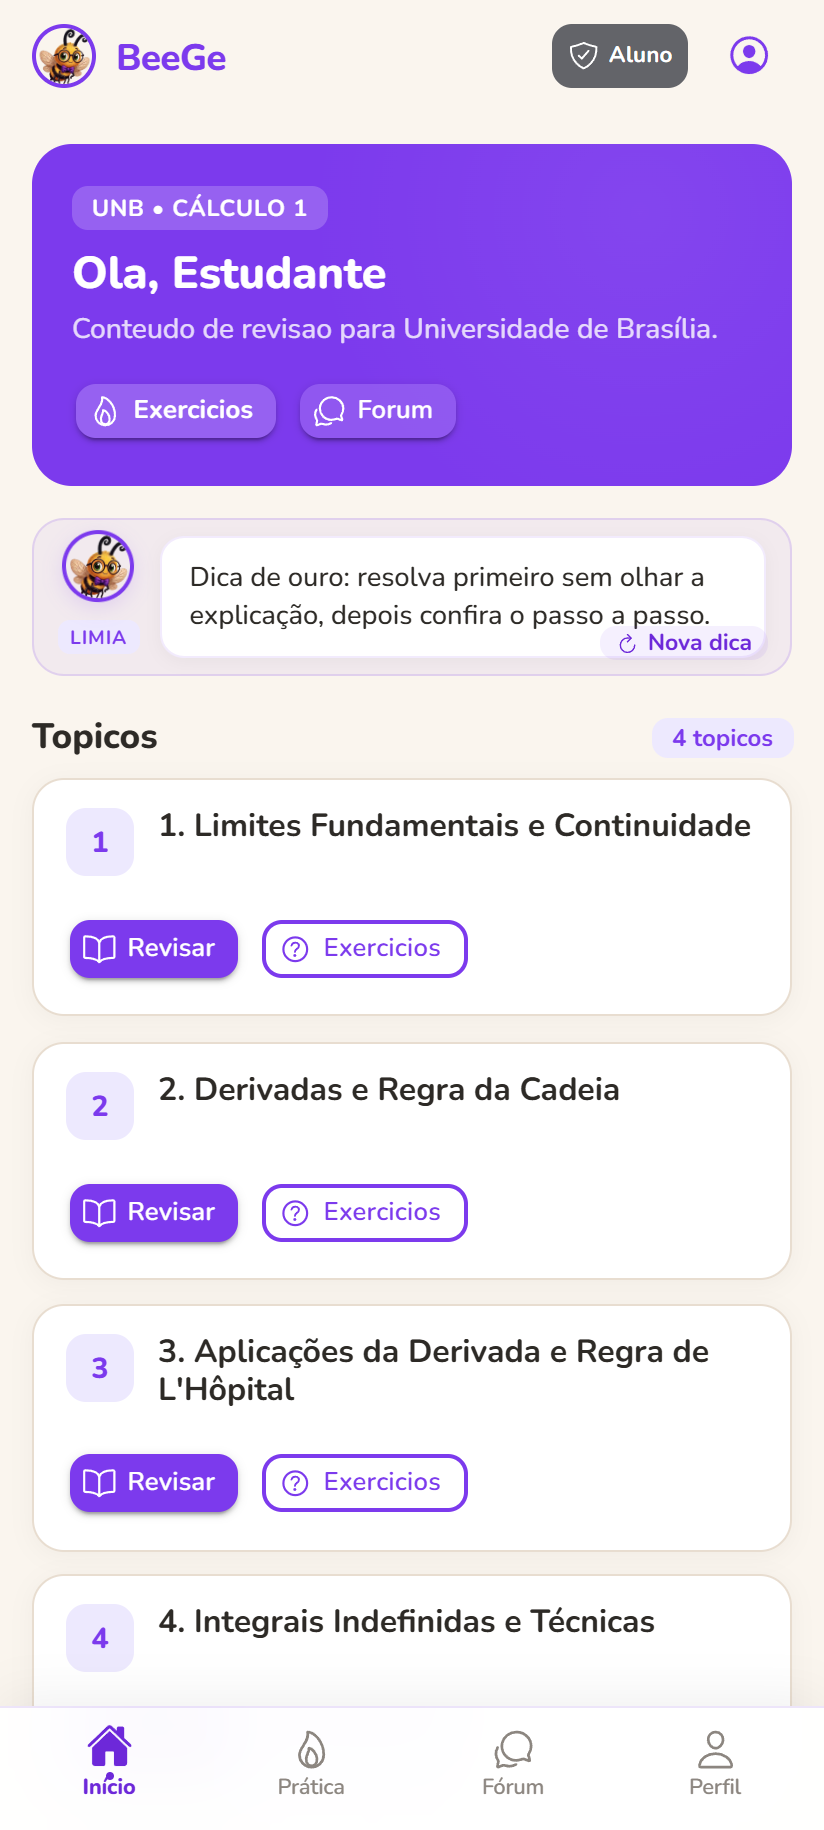
\includegraphics[height=9.6cm, keepaspectratio]{screenshots/01_dashboard.png}
	\caption{Dashboard com m\'{o}dulos e streaks}
	\label{fig:dashboard}
\end{minipage}
\hfill
\begin{minipage}{0.48\textwidth}
	\centering
	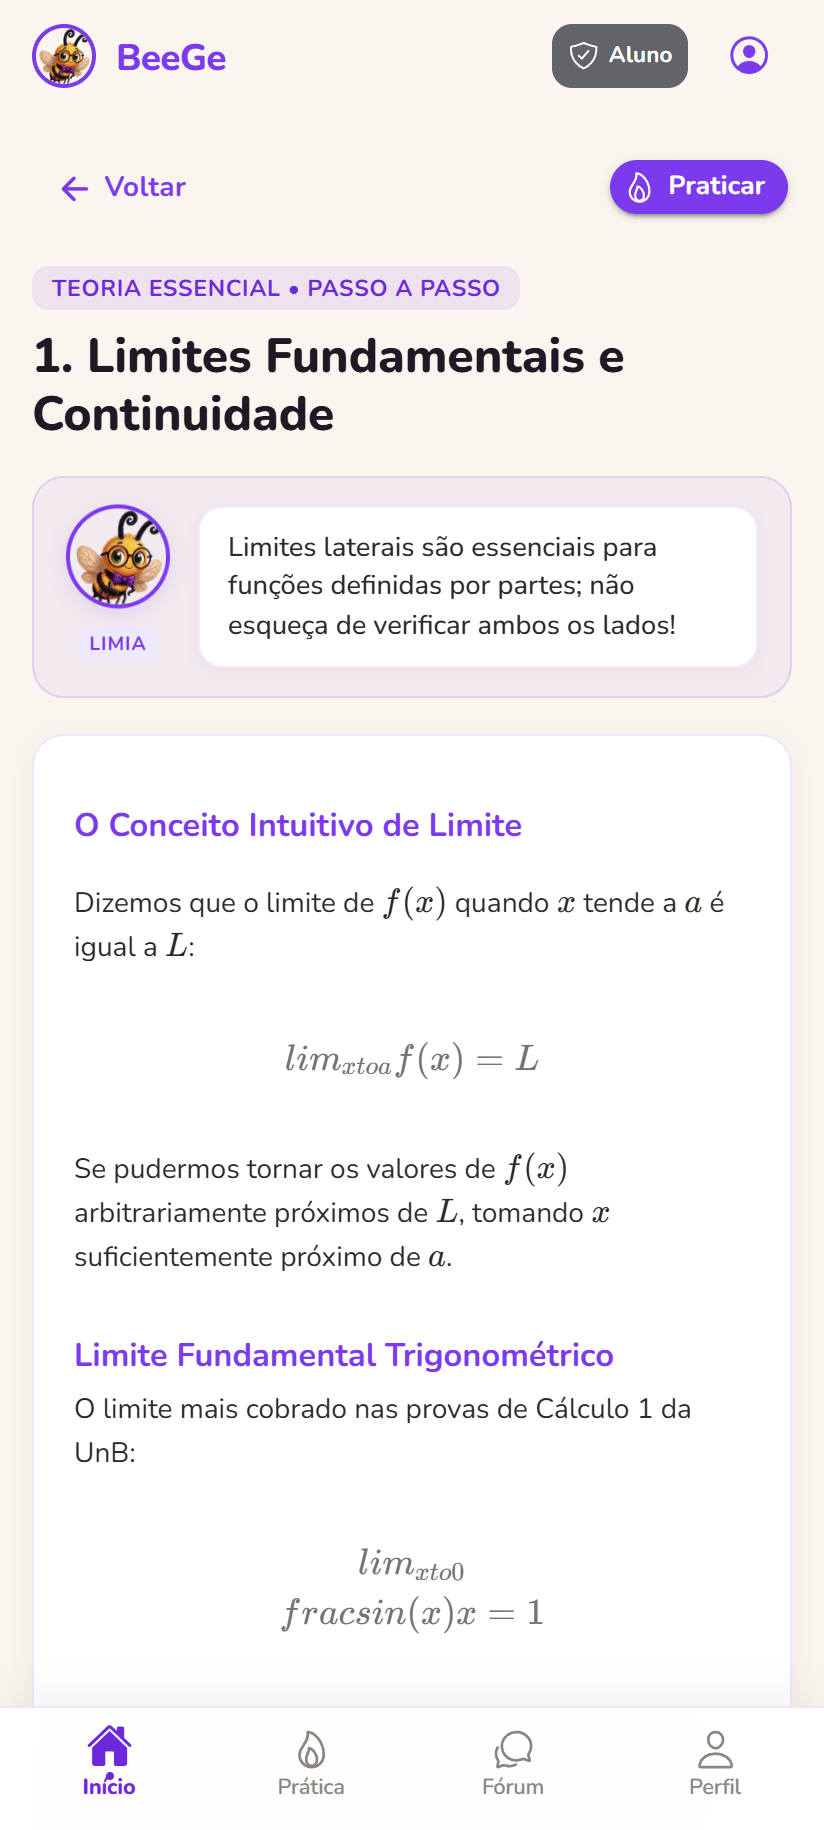
\includegraphics[height=9.6cm, keepaspectratio]{screenshots/02_teoria.png}
	\caption{Tela de revis\~{a}o te\'{o}rica}
	\label{fig:teoria}
\end{minipage}
\end{figure}

\begin{figure}[H]
\centering
\begin{minipage}{0.48\textwidth}
	\centering
	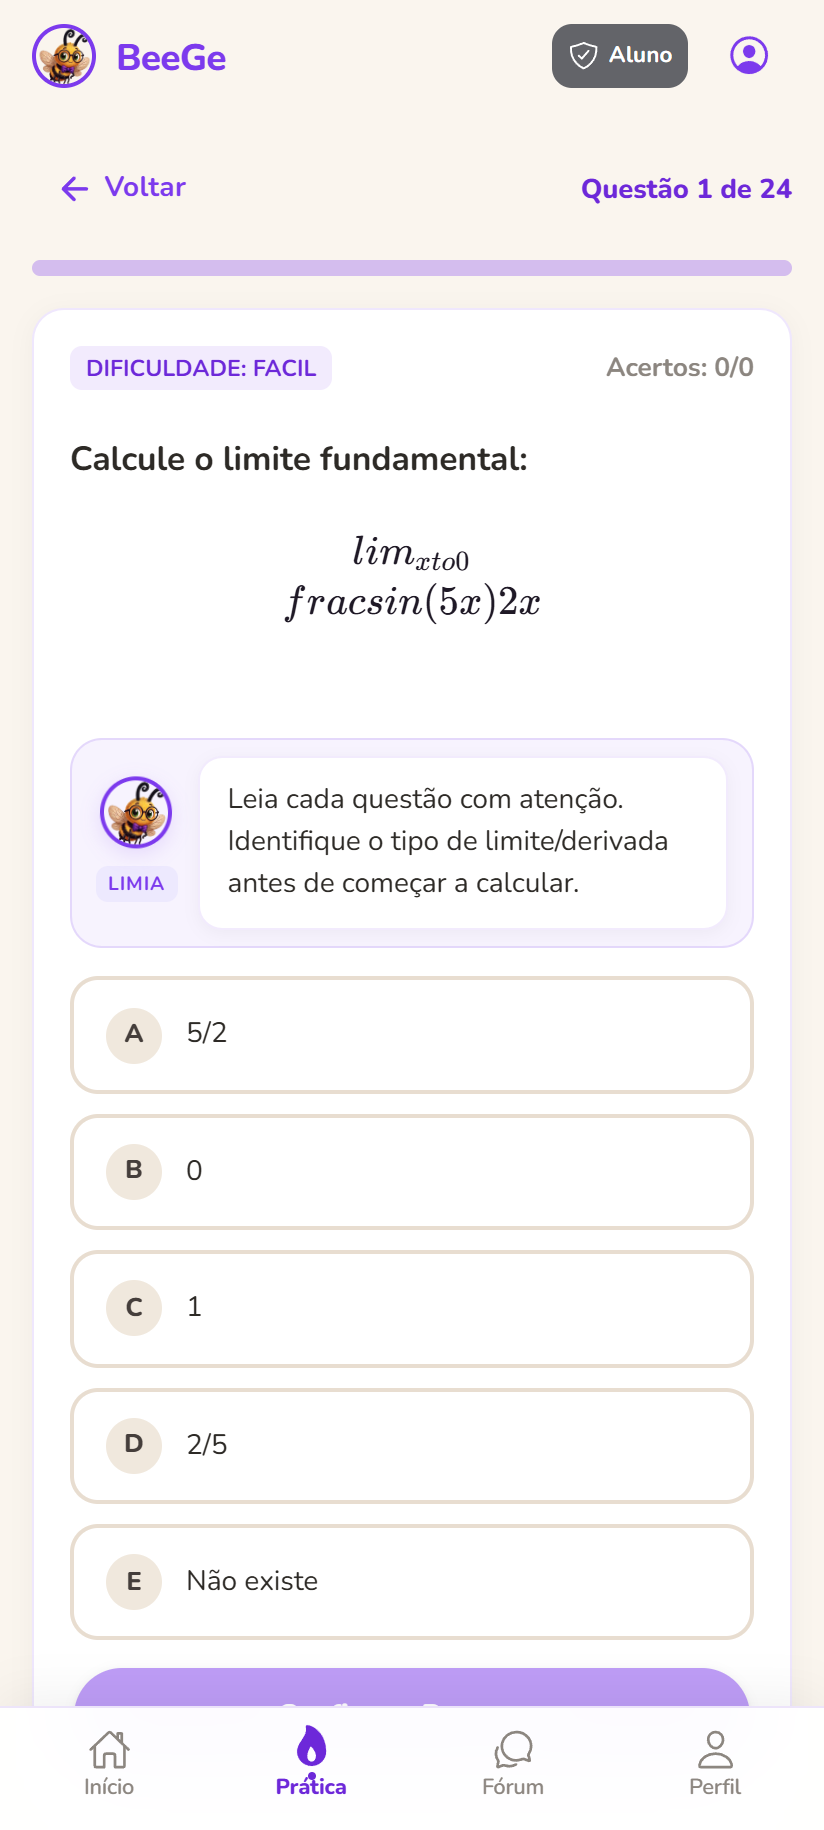
\includegraphics[height=8.3cm, keepaspectratio]{screenshots/03_pratica.png}
	\caption{Exerc\'{i}cio com resolu\c{c}\~{a}o passo a passo}
	\label{fig:pratica}
\end{minipage}
\hfill
\begin{minipage}{0.48\textwidth}
	\centering
	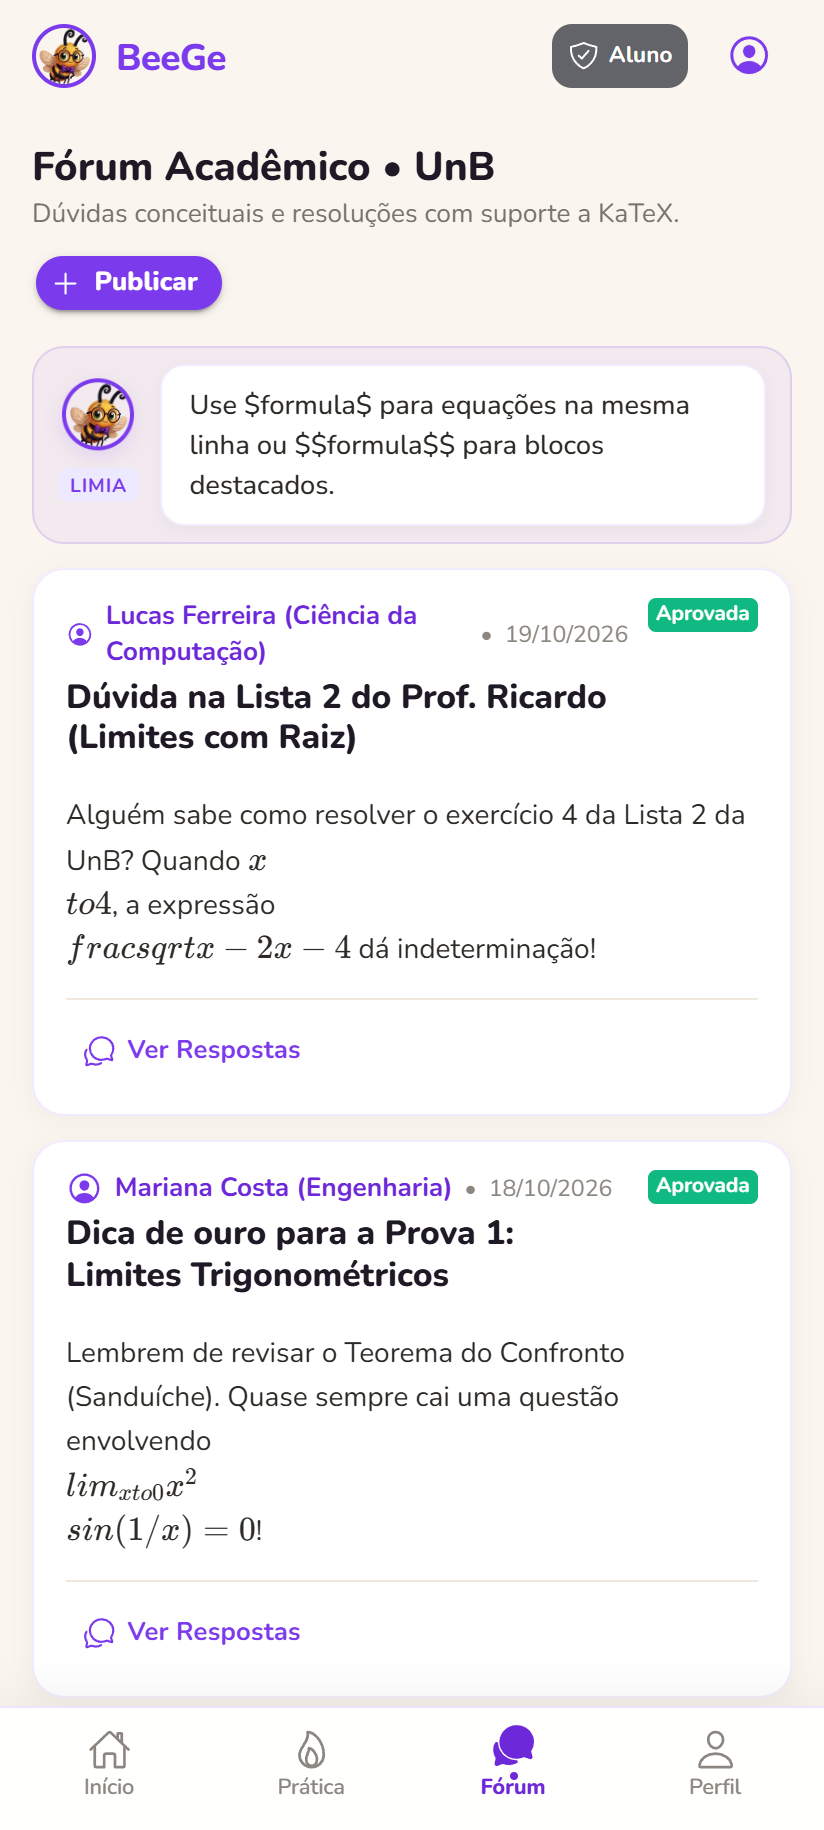
\includegraphics[height=8.3cm, keepaspectratio]{screenshots/04_forum.png}
	\caption{F\'{o}rum de d\'{u}vidas}
	\label{fig:forum}
\end{minipage}

\vspace{10pt}

\begin{minipage}{0.48\textwidth}
	\centering
	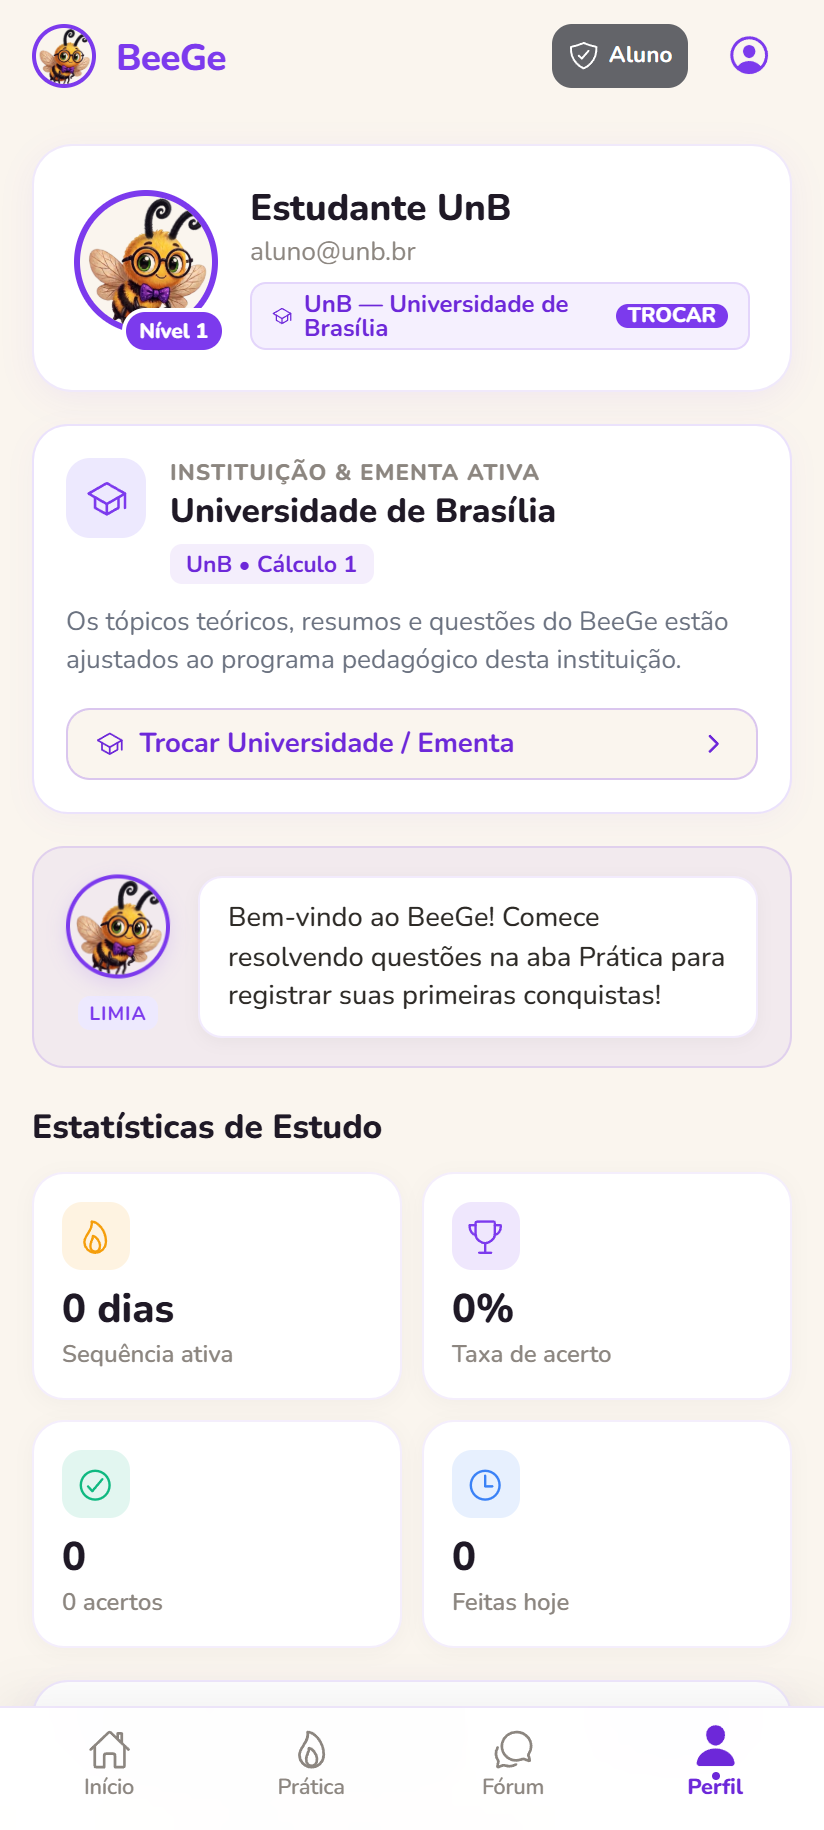
\includegraphics[height=8.3cm, keepaspectratio]{screenshots/05_perfil.png}
	\caption{Perfil com n\'{i}vel e estat\'{i}sticas}
	\label{fig:perfil}
\end{minipage}
\hfill
\begin{minipage}{0.48\textwidth}
	\centering
	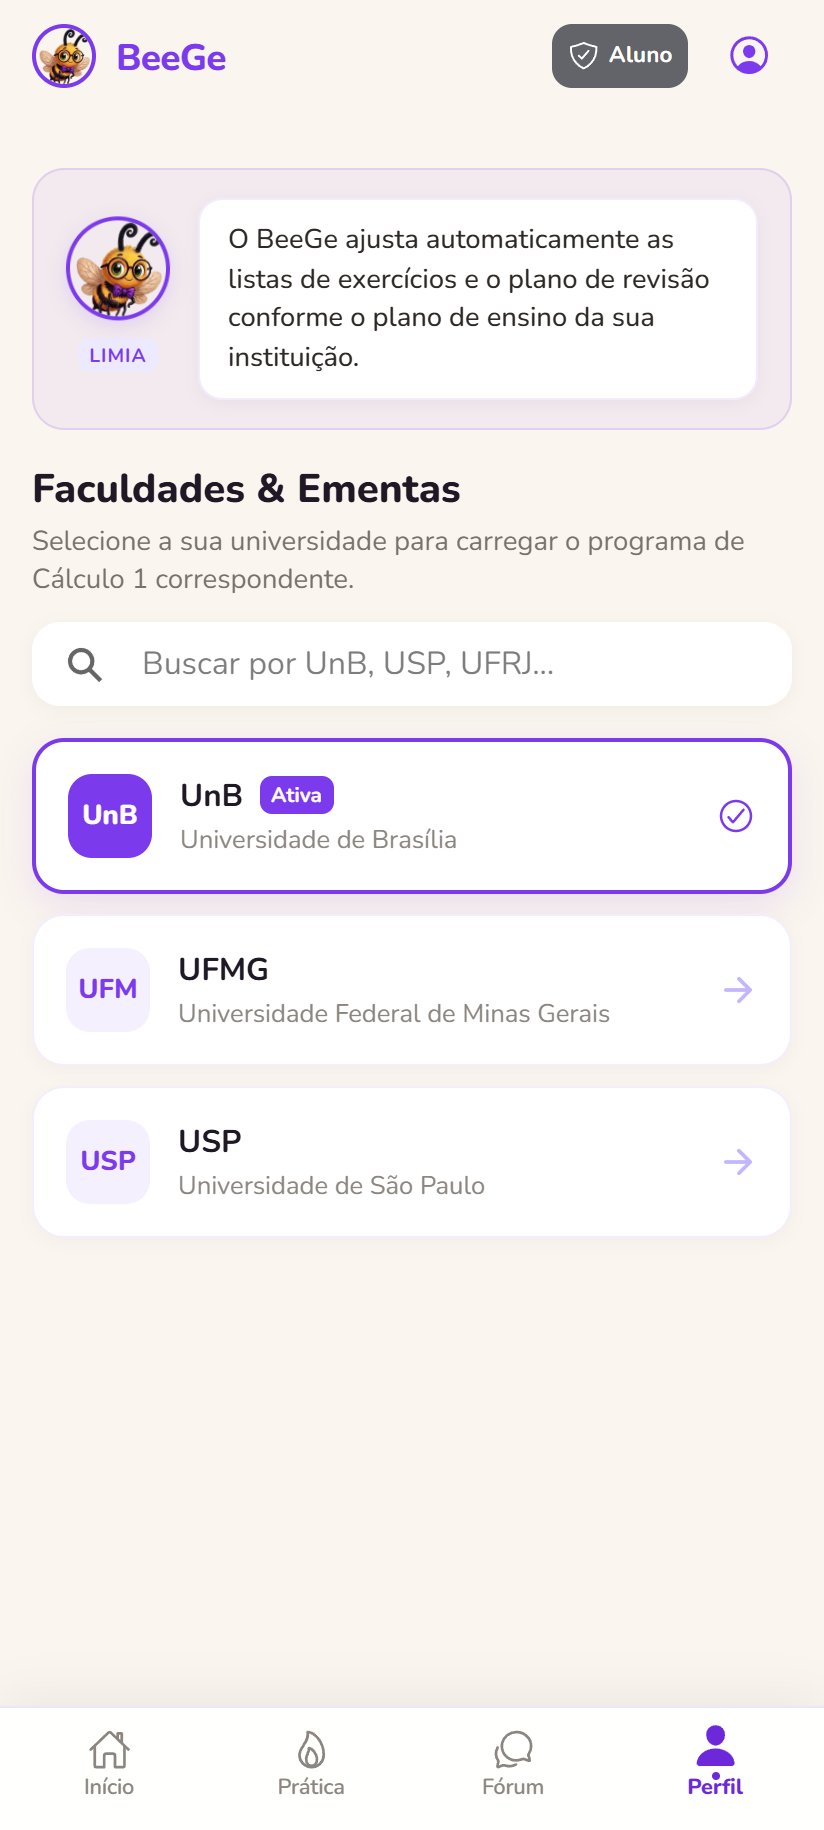
\includegraphics[height=8.3cm, keepaspectratio]{screenshots/06_universidades.png}
	\caption{Sele\c{c}\~{a}o de universidade}
	\label{fig:universidades}
\end{minipage}
\end{figure}

\newpage
% ========================================================================
%  12. MODELO DE NEGOCIO
% ========================================================================
\section{Vis\~{a}o de Neg\'{o}cio}

\subsection{Do MVP ao Produto Final}

Desde o come\c{c}o, pensei o BeeGe para funcionar com v\'{a}rias universidades ao mesmo tempo. Cada faculdade tem seus pr\'{o}prios t\'{o}picos, quest\~{o}es e f\'{o}rum, tudo separado. Essa organiza\c{c}\~{a}o permite que o MVP vire um produto comercial de verdade:

\begin{itemize}[leftmargin=2cm]
  \item Cada universidade pode montar suas quest\~{o}es e trilhas do jeito que quiser, de acordo com a grade curricular.
  \item Monitores e professores conseguem criar e moderar conte\'{u}do sem precisar de mim.
  \item Adicionar uma nova faculdade \'{e} simples --- n\~{a}o precisa mudar o c\'{o}digo do app.
\end{itemize}

\subsection{Crescimento Futuro}

A estrutura do app permite expandir para outras mat\'{e}rias no futuro:

\begin{itemize}[leftmargin=2cm]
  \item C\'{a}lculo~2
  \item C\'{a}lculo~3
  \item \'{A}lgebra Linear
  \item Equa\c{c}\~{o}es Diferenciais
\end{itemize}

\subsection{Impacto que eu quero causar}

\begin{destaque}[Impacto Esperado]
Minha vis\~{a}o \'{e} que o BeeGe ajude milhares de estudantes de C\'{a}lculo~1 pelo Brasil, oferecendo uma ferramenta de revis\~{a}o acess\'{i}vel, gamificada e que respeita a realidade de cada faculdade. Al\'{e}m de ajudar os alunos, esse projeto \'{e} a realiza\c{c}\~{a}o de um sonho empreendedor que nasceu dentro do NaPr\'{a}tica.
\end{destaque}

% ========================================================================
%  13. RESULTADOS
% ========================================================================
\section{Resultados Alcan\c{c}ados}

\begin{table}[H]
\centering
\small
\renewcommand{\arraystretch}{1.15}
\caption{O que foi alcan\c{c}ado no MVP}
\begin{tabularx}{\textwidth}{X l l}
\toprule
\textbf{Meta} & \textbf{O que eu queria} & \textbf{O que consegui} \\
\midrule
T\'{o}picos de C\'{a}lculo~1 & Pelo menos 4 & Atingido \\
Quest\~{o}es com resolu\c{c}\~{a}o completa & Pelo menos 20 & 24 (superei a meta) \\
Testes automatizados & Cobrir as partes principais & 17 testes, todos passaram \\
App compilando & Sem erros & Atingido \\
App mobile & Android/iOS & Funcionando \\
Documenta\c{c}\~{a}o & Tudo documentado & 12 documentos produzidos \\
\bottomrule
\end{tabularx}
\end{table}

% ========================================================================
%  14. DOCUMENTACAO
% ========================================================================
\section{Documenta\c{c}\~{a}o Produzida}

Ao longo do desenvolvimento, produzi 12 documentos que registram todas as decis\~{o}es e detalhes do projeto:

\begin{table}[H]
\centering
\small
\renewcommand{\arraystretch}{1.12}
\caption{Documentos do projeto}
\begin{tabularx}{\textwidth}{l X}
\toprule
\textbf{Documento} & \textbf{O que cont\'{e}m} \\
\midrule
Vis\~{a}o do Produto & O problema, a solu\c{c}\~{a}o e os objetivos do BeeGe \\
Canvas MVP & Resumo do produto m\'{i}nimo vi\'{a}vel em uma p\'{a}gina \\
Personas & 3 perfis de usu\'{a}rio (Calouro, Veterana, Monitor) \\
Requisitos & O que o app precisa fazer e como precisa funcionar \\
Backlog & As 18 hist\'{o}rias de usu\'{a}rio organizadas em 6 grupos \\
Arquitetura & Como o sistema \'{e} organizado por dentro \\
Diagramas & Desenhos t\'{e}cnicos mostrando como as partes se conectam \\
Metodologia & Como organizei o trabalho em sprints \\
Cronograma & As 5 sprints com datas e entregas \\
Qualidade & Como garanti que o app funciona direito \\
Riscos & O que poderia dar errado e como me preparei \\
Guia de Contribui\c{c}\~{a}o & Como algu\'{e}m poderia contribuir com o c\'{o}digo \\
\bottomrule
\end{tabularx}
\end{table}

\newpage
% ========================================================================
%  15. CONCLUSAO
% ========================================================================
\section{Conclus\~{a}o}

Desenvolver o BeeGe em 30 dias foi muito mais do que um desafio t\'{e}cnico --- foi um \textbf{salto pessoal}. O projeto me mostrou que, com planejamento e as ferramentas certas, d\'{a} para sair da ideia e chegar num produto funcionando em pouco tempo.

O que eu entreguei:

\begin{itemize}[leftmargin=2cm]
  \item Um app que resolve um problema real de milhares de estudantes.
  \item Uma estrutura pronta para crescer e atender v\'{a}rias universidades.
  \item Documenta\c{c}\~{a}o completa de todo o processo.
  \item Testes que comprovam que o app funciona.
  \item Uma identidade visual pr\'{o}pria com a mascote Limia.
\end{itemize}

Mais do que um app, o BeeGe \'{e} a prova de que eu tive coragem de empreender. Um passo que nasceu dentro do NaPr\'{a}tica e que agora est\'{a} pronto para virar uma empresa de verdade, capaz de mudar a forma como estudantes revisam e aprendem C\'{a}lculo~1.

\vspace{1cm}

\begin{center}
\textcolor{beegePurple}{\rule{0.5\textwidth}{1pt}}\\[0.5cm]
\textit{``Me desafiei a fazer algo que eu sempre quis, mas n\~{a}o tinha coragem: empreender.''}\\[0.3cm]
\textbf{Gabriel Monteiro, 2026}\\[0.5cm]
\textcolor{beegePurple}{\rule{0.5\textwidth}{1pt}}
\end{center}
\newpage
% ========================================================================
%  REFERENCIAS
% ========================================================================
\addcontentsline{toc}{section}{Refer\^{e}ncias}
{
\begin{spacing}{1.08}
\begin{thebibliography}{99}
\setlength{\itemsep}{2pt}

\bibitem{stewart2016}
STEWART, J. \textit{C\'{a}lculo}. 8. ed. S\~{a}o Paulo: Cengage Learning, 2016.

\bibitem{ries2011}
RIES, E. \textit{The Lean Startup}. New York: Crown Business, 2011.

\bibitem{supabase2024}
SUPABASE INC. \textit{Supabase Documentation}. 2024. Dispon\'{i}vel em: \url{https://supabase.com/docs}. Acesso em: out. 2026.

\bibitem{ionic2024}
IONIC TEAM. \textit{Ionic Framework Documentation}. 2024. Dispon\'{i}vel em: \url{https://ionicframework.com/docs}. Acesso em: out. 2026.

\bibitem{katex2024}
KHAN ACADEMY. \textit{KaTeX: The fastest math typesetting library for the web}. 2024. Dispon\'{i}vel em: \url{https://katex.org/}. Acesso em: out. 2026.

\bibitem{capacitor2024}
IONIC TEAM. \textit{Capacitor: Cross-platform Native Runtime for Web Apps}. 2024. Dispon\'{i}vel em: \url{https://capacitorjs.com/docs}. Acesso em: out. 2026.

\end{thebibliography}
\end{spacing}
}

\vspace{0.8cm}
\appendix
\section{Declara\c{c}\~{a}o de Uso de Intelig\^{e}ncia Artificial}
Em transpar\^{e}ncia, declaro que usei ferramentas de IA durante o desenvolvimento:
\begin{itemize}
    \item \textbf{Ferramenta:} Gemini 3.8 (Google DeepMind).
    \item \textbf{Para qu\^{e}:} Ajuda na corre\c{c}\~{a}o de testes e c\'{o}digo, gera\c{c}\~{a}o de componentes Ionic/React, revis\~{a}o de f\'{o}rmulas matem\'{a}ticas e cria\c{c}\~{a}o da mascote Limia.
    \item \textbf{Revis\~{a}o:} Todo c\'{o}digo e conte\'{u}do gerado foi revisado, testado e validado por mim antes de entregar no projeto.
\end{itemize}

\end{document}
